\documentclass[14pt]{extbook}
\usepackage{multicol, enumerate, enumitem, hyperref, color, soul, setspace, parskip, fancyhdr} %General Packages
\usepackage{amssymb, amsthm, amsmath, bbm, latexsym, units, mathtools} %Math Packages
\everymath{\displaystyle} %All math in Display Style
% Packages with additional options
\usepackage[headsep=0.5cm,headheight=12pt, left=1 in,right= 1 in,top= 1 in,bottom= 1 in]{geometry}
\usepackage[usenames,dvipsnames]{xcolor}
\usepackage{dashrule}  % Package to use the command below to create lines between items
\newcommand{\litem}[1]{\item#1\hspace*{-1cm}\rule{\textwidth}{0.4pt}}
\pagestyle{fancy}
\lhead{Progress Quiz 4}
\chead{}
\rhead{Version B}
\lfoot{8448-1521}
\cfoot{}
\rfoot{Fall 2020}
\begin{document}

\begin{enumerate}
\litem{
Choose the graph of the equation below.\[ f(x) = - \sqrt[3]{x - 8} - 5 \]\begin{enumerate}[label=\Alph*.]
\begin{multicols}{2}\item 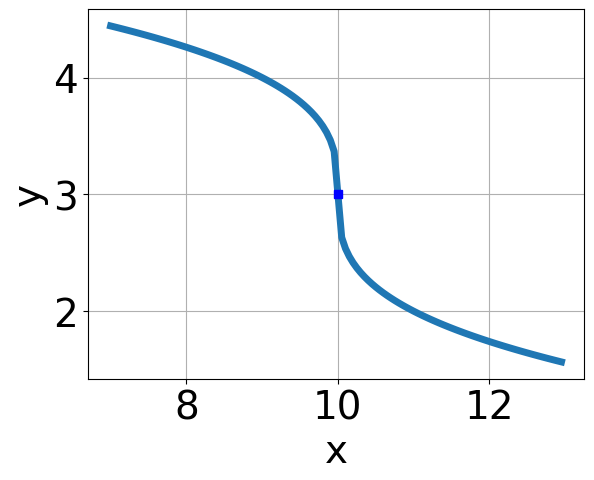
\includegraphics[width = 0.3\textwidth]{../Figures/radicalEquationToGraphAB.png}\item 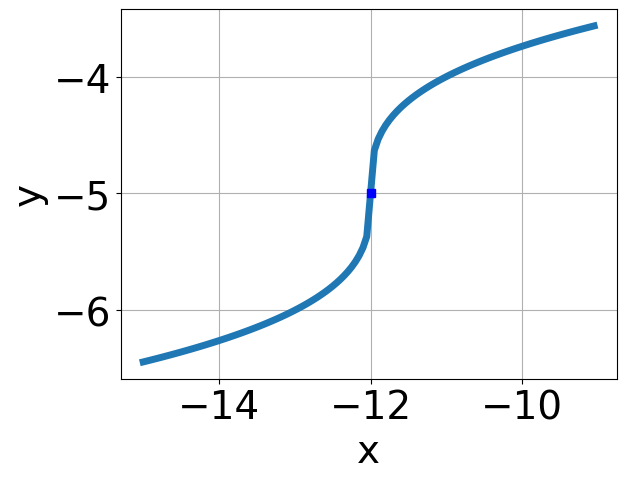
\includegraphics[width = 0.3\textwidth]{../Figures/radicalEquationToGraphBB.png}\item 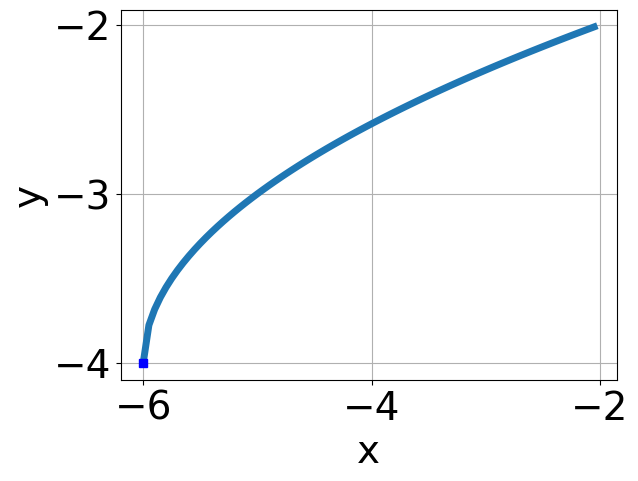
\includegraphics[width = 0.3\textwidth]{../Figures/radicalEquationToGraphCB.png}\item 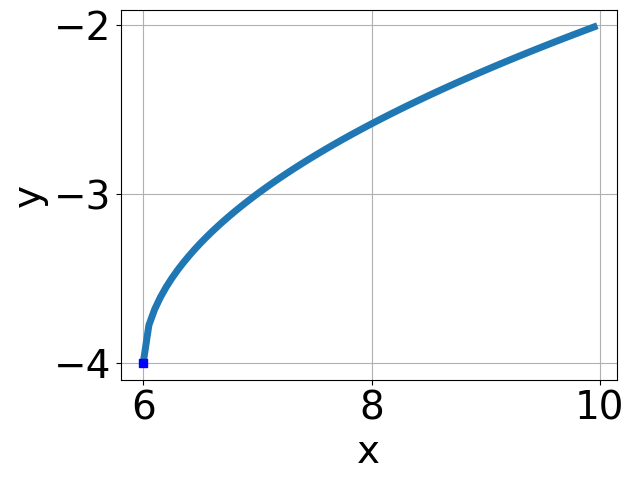
\includegraphics[width = 0.3\textwidth]{../Figures/radicalEquationToGraphDB.png}\end{multicols}\item None of the above.
\end{enumerate} }
\litem{
Solve the radical equation below. Then, choose the interval(s) that the solution(s) belongs to.\[ \sqrt{-8 x + 7} - \sqrt{8 x + 4} = 0 \]\begin{enumerate}[label=\Alph*.]
\item \( \text{All solutions lead to invalid or complex values in the equation.} \)
\item \( x_1 \in [-0.39, 0.67] \text{ and } x_2 \in [-6.12,1.88] \)
\item \( x \in [-0.39,0.67] \)
\item \( x_1 \in [-1.29, -0.24] \text{ and } x_2 \in [-6.12,1.88] \)
\item \( x \in [0.34,1.19] \)

\end{enumerate} }
\litem{
Choose the equation of the function graphed below.
\begin{center}
    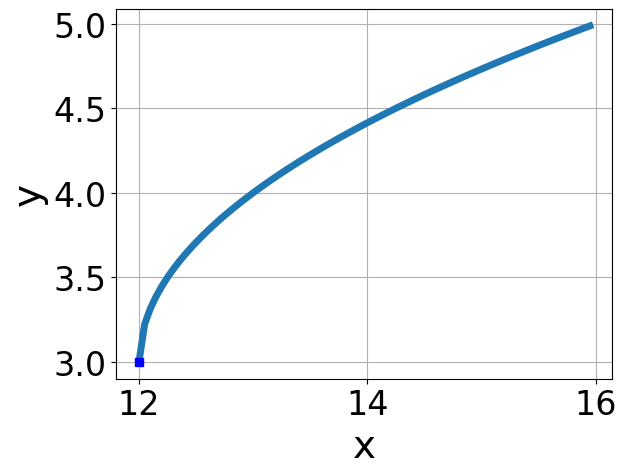
\includegraphics[width=0.5\textwidth]{../Figures/radicalGraphToEquationCopyB.png}
\end{center}
\begin{enumerate}[label=\Alph*.]
\item \( f(x) = \sqrt[3]{x - 6} - 5 \)
\item \( f(x) = \sqrt[3]{x + 6} - 5 \)
\item \( f(x) = - \sqrt[3]{x + 6} - 5 \)
\item \( f(x) = - \sqrt[3]{x - 6} - 5 \)
\item \( \text{None of the above} \)

\end{enumerate} }
\litem{
Solve the radical equation below. Then, choose the interval(s) that the solution(s) belongs to.\[ \sqrt{12 x^2 + 81} - \sqrt{72 x} = 0 \]\begin{enumerate}[label=\Alph*.]
\item \( x \in [3.5,6.5] \)
\item \( x_1 \in [1.5, 3.5] \text{ and } x_2 \in [4.5,6.5] \)
\item \( x \in [1.5,3.5] \)
\item \( x_1 \in [-9.5, -2.5] \text{ and } x_2 \in [-4.5,2.5] \)
\item \( \text{All solutions lead to invalid or complex values in the equation.} \)

\end{enumerate} }
\litem{
Solve the radical equation below. Then, choose the interval(s) that the solution(s) belongs to.\[ \sqrt{9 x - 6} - \sqrt{3 x + 6} = 0 \]\begin{enumerate}[label=\Alph*.]
\item \( x_1 \in [-2.56, -1.81] \text{ and } x_2 \in [-0.33,1.67] \)
\item \( x_1 \in [0.32, 1.17] \text{ and } x_2 \in [1,6] \)
\item \( x \in [1.63,2.6] \)
\item \( \text{All solutions lead to invalid or complex values in the equation.} \)
\item \( x \in [-0.88,0.49] \)

\end{enumerate} }
\litem{
Choose the graph of the equation below.\[ f(x) = - \sqrt{x + 12} - 3 \]\begin{enumerate}[label=\Alph*.]
\begin{multicols}{2}\item 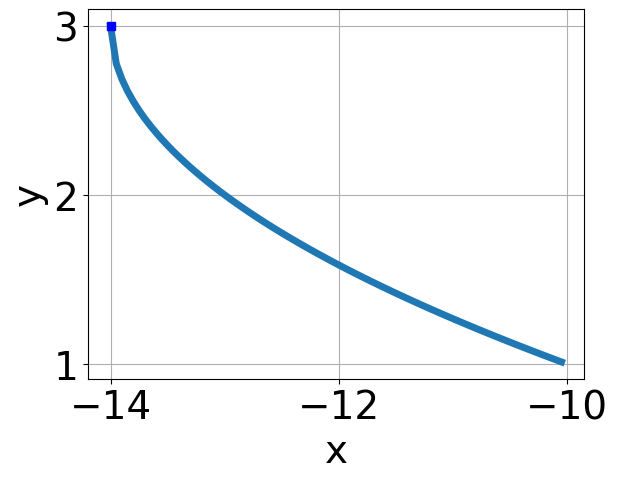
\includegraphics[width = 0.3\textwidth]{../Figures/radicalEquationToGraphCopyAB.png}\item 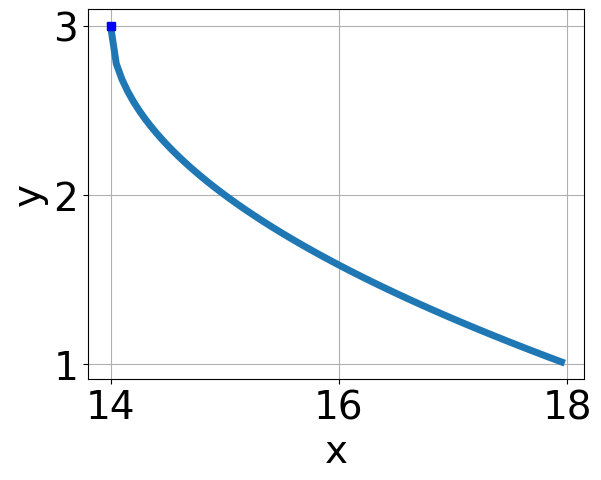
\includegraphics[width = 0.3\textwidth]{../Figures/radicalEquationToGraphCopyBB.png}\item 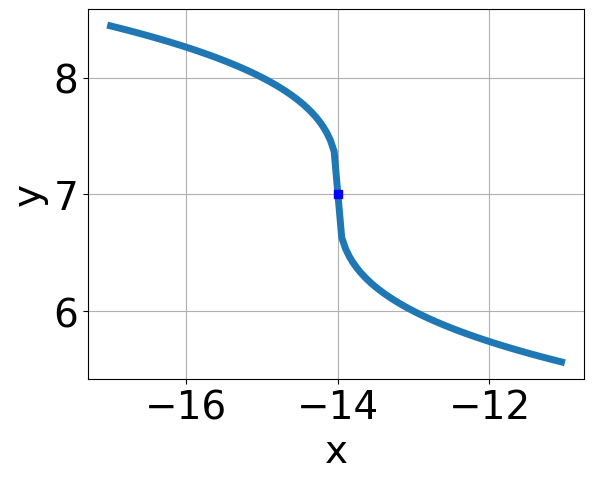
\includegraphics[width = 0.3\textwidth]{../Figures/radicalEquationToGraphCopyCB.png}\item 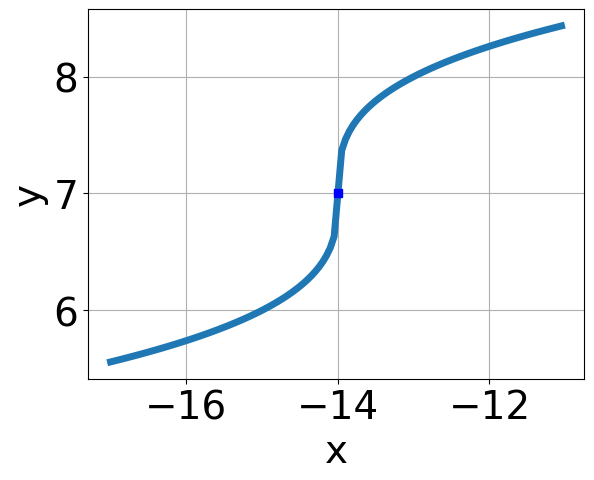
\includegraphics[width = 0.3\textwidth]{../Figures/radicalEquationToGraphCopyDB.png}\end{multicols}\item None of the above.
\end{enumerate} }
\litem{
Solve the radical equation below. Then, choose the interval(s) that the solution(s) belongs to.\[ \sqrt{-54 x^2 - 30} - \sqrt{-81 x} = 0 \]\begin{enumerate}[label=\Alph*.]
\item \( x \in [0.44,0.73] \)
\item \( x_1 \in [-0.8, -0.43] \text{ and } x_2 \in [-1.9,-0.3] \)
\item \( x \in [0.76,0.96] \)
\item \( x_1 \in [0.44, 0.73] \text{ and } x_2 \in [0.3,2.2] \)
\item \( \text{All solutions lead to invalid or complex values in the equation.} \)

\end{enumerate} }
\litem{
What is the domain of the function below?\[ f(x) = \sqrt[3]{-4 x - 5} \]\begin{enumerate}[label=\Alph*.]
\item \( \text{The domain is } (-\infty, a], \text{   where } a \in [-0.91, -0.61] \)
\item \( (-\infty, \infty) \)
\item \( \text{The domain is } [a, \infty), \text{   where } a \in [-2.88, -1.23] \)
\item \( \text{The domain is } (-\infty, a], \text{   where } a \in [-2.24, -0.81] \)
\item \( \text{The domain is } [a, \infty), \text{   where } a \in [-1.01, -0.02] \)

\end{enumerate} }
\litem{
Choose the equation of the function graphed below.
\begin{center}
    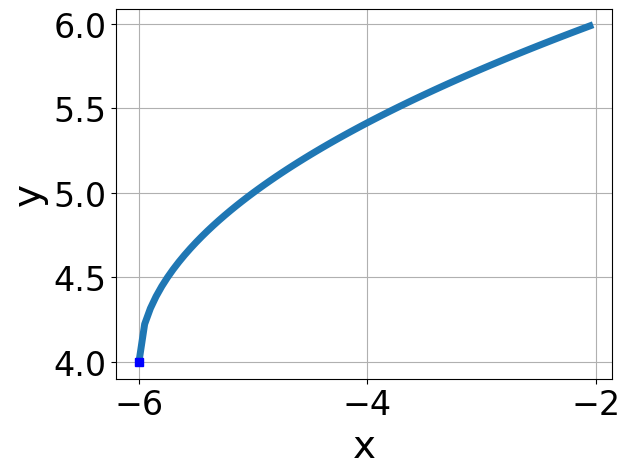
\includegraphics[width=0.5\textwidth]{../Figures/radicalGraphToEquationB.png}
\end{center}
\begin{enumerate}[label=\Alph*.]
\item \( f(x) = - \sqrt{x - 10} - 6 \)
\item \( f(x) = \sqrt{x - 10} - 6 \)
\item \( f(x) = \sqrt{x + 10} - 6 \)
\item \( f(x) = - \sqrt{x + 10} - 6 \)
\item \( \text{None of the above} \)

\end{enumerate} }
\litem{
What is the domain of the function below?\[ f(x) = \sqrt[8]{7 x + 4} \]\begin{enumerate}[label=\Alph*.]
\item \( (-\infty, a], \text{where } a \in [-3.3, -1.17] \)
\item \( (-\infty, \infty) \)
\item \( (-\infty, a], \text{where } a \in [-0.66, -0.36] \)
\item \( [a, \infty), \text{where } a \in [-4.1, -0.58] \)
\item \( [a, \infty), \text{ where } a \in [-1.02, -0.28] \)

\end{enumerate} }
\end{enumerate}

\end{document}